\documentclass[12pt]{book}
\usepackage{mathtools}
\usepackage{graphicx}
\usepackage{subcaption}
\usepackage[utf8]{inputenc}
\usepackage{float}
\usepackage{tabularx}
\usepackage{chngpage}
\usepackage{amsthm}
\usepackage{mathtools}
\usepackage{amsfonts}
\usepackage{tikz}
\usepackage{amssymb}
\usepackage{gensymb}
\usepackage{wrapfig}
\usepackage{enumerate}
\usepackage{braket}
\usepackage{pgfplots}
\usepackage{bbm}
\usepackage{fancyhdr}
\usepackage{emptypage}


%\numberwithin{equation}{section}
\newcommand{\R}{\mathbb{R}}
\newcommand{\F}{\mathcal{F}}
\renewcommand{\L}{\mathcal{L}}
\newcommand{\C}{\mathbb{C}}
\renewcommand{\H}{\mathcal{H}}
\newcommand{\Sum}{\sum_{n=0}^\infty}
\newcommand{\Res}[1]{\text{Res}f(z)\Big|_{#1}}
\newcommand{\vettore}[1]{\overrightarrow{#1}}
\newcommand{\p}{\mathbf{p}}
\newcommand{\x}{\mathbf{x}}
\renewcommand{\r}{\mathbf{r}}


\usepackage[a4paper, inner=1.5cm, outer=3cm, top=3cm, 
bottom=3cm, bindingoffset=1cm,headheight=110pt]{geometry} 


\pagestyle{fancy}
\fancyhf{}
\fancyhead[LE]{\leftmark}
\fancyhead[RO]{\rightmark}
\fancyfoot[C]{\thepage}
\begin{document}
\begin{titlepage}
  \pagestyle{empty}

  \begin{center}
    {\bfseries
      \Large {\huge U}NIVERSITY OF {\huge T}RENTO}

    \vspace{0.2cm}

    {\Large Department of Physics}

    \vspace{0.5cm}

    \begin{center}
      
\includegraphics[width=0.3\textwidth]{img/logo_unitn.png}
    \end{center}

    \vspace{0.5cm}

    {\bfseries \Large Degree course in Physics}

    \vspace{0.3cm}
    \line(1,0){338}
    \vspace{0.3cm}

    {\Large Final Thesis}

    \vspace{2.5cm}

    {\huge \textsc{Generation and manipulation of}}

    \vspace{0.4cm}

    {\huge \textsc{entangled photon pairs in}}

     \vspace{0.4cm}

     {\huge \textsc{coupled resonators}}
    

    \vspace{3.0cm}


    \large
    \begin{center}
      \begin{tabular}{ccc}
        {\bfseries Supervisor} &
        \hspace{5cm}
        {\bfseries Candidate} \\

        Prof. Lorenzo Pavesi &
        \hspace{5cm} Marco Canteri \\


      \end{tabular}
    \end{center}
    \vspace{2cm}

    {\bfseries \large Academic year 2016-2017}
    \vfill
  \end{center}
\end{titlepage}

\tableofcontents
\chapter{Introduction}
The aim of this thesis is to describe a theoretical model for the generation of entangled photons inside silicon optic chips. In particular, the structure I am going to study is composed by two microrings side coupled to two waveguides. Due to interference, the electric field inside a ring in enhanced and a great amount of energy is stored inside, which leads to non linear effects. Imposing a phase matching condition it is possible to select which non linear effect is more efficient and therefore which one is significant. Generation of entangled photons is possible by means of Spontaneous Four Wave Mixing, a third order non-linear effect of silicon.
In addition to this, the main advantage of using two coupled resonators is that it is possibile to change the phases of the fields in the waveguides between the rings, and I will show how this can be exploited in order to build a tunable device where we can manipulate the output state of the generated photons.
\\
In order to describe this process, the first chapter gives a description of the needed basic structures, microrings and waveguides and how we can describe their behaviour using a mathematical formalism. The second chapter is devoted to the explanation of the physics behind the phenomena and the mathematics which can be used to carry out the calculation. Finally in the last chapter the model and the results are presented.
\section{Integrated optics}
The microelectronics has been widely succesful and it was a revolution that changed our daily life and work; nowadays microelectronics is present almost everywhere. The great success of these technologies is due to many reasons. One of them is the computational power of a small chip which by Moore's law is predicted to be doubled every two years. The prediction still holds today, but we are reaching a saturation point: improvements were possible by increasing the clock frequencies of the processing units, but this kind of improvement faces several problems, such as heating power, antenna effects and RC time delays. Therefore, in order to keep the improvements going, the approach used is now to increase the number of processing units, but the problems are still present, they are only changed. The cores need to communicate with each other, so the problem is to realise efficient communication with high bandwidth and low power consumption. Photonics is a platform that can be used to achieve such goal: with light is possible to realize ultra-high speed switches, it has low power consumption and it doesn't have electromagnetic noise. Several platforms have been developed with different media, such as silicon, lithium niobate, gallium arsenide. Since the electronics industry is based on silicon, Silicon-on-Insulator (SOI) photonics is a promising platform to build optical chips. Indeed, the technology used for the fabrication of silicon chips is well studied and understood, it has reached a high level of sophistication and the industries and the infrastructures already exist. Futhermore silicon photonic is compatible with CMOS technology used in electronic chips, hence hybrid chips with electronics and photonics can be realised. Another important feature of silicon is its transparency at the important Telecom wavelengths (1300-1600 nm), which allows the fabrication of optic circuits with very low power losses. The aim of silicon photonics is to follow the philosophy behind microelectronics: small chips composed by few building blocks that can be used to build different devices changing the topology of the chip, and to realise these building blocks with as few materials as possible with a standard established among manifacturers.\\
From the point of view of quantum mechanics, light is composed by elementary particles called photons. Photons have quantum properties, hence it is possible to build quantum devices using the already implemented building blocks. Photons can be used to represent quantum bits and due to their low decoherence effects, they are an attractive approch to quantum information processing. Quantum technologies can drastically improve some tasks in computation, measurement and communication , and quantum silicon photonics is a great platform for developing such technologies on a single chip. 


\section{Waveguides}
A silicon optical chip is realised with three different layers as depicted in figure \ref{SOIstructure}. At the bottom we can find the substrate, a silicon layer which provides a base and a stable structure for the chip; just above it there is a layer made of silicon dioxide called cladding and finally at the top there is another silicon layer called the core. The thickness of the substrate is in the order of $700\, \mu m $ and the cladding in the order of some $\mu m$, while the core has a height in the order of a few hundred $nm$. The refractive index of silicon is $n_{Si} \simeq 3.5$, in the range of the Telecom wavelengths, while the refractive index of silicon dioxide is $n_{SiO_2}\simeq 1.54$, in the same range; this allows the confinement of light in the core layer by total internal refraction. Exactly like in optical fibers, when the light, travelling in the core layer, reaches the boundaries with the cladding or with the air (refractive index $\simeq 1$) is reflected back if the angle of incidence is greater than a critical angle. 
\begin{figure}
\centering
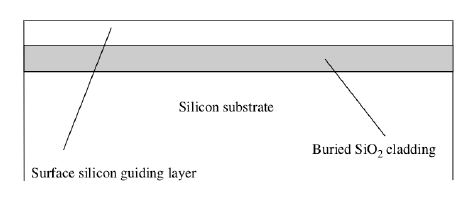
\includegraphics[width = .7\textwidth]{img/SOIstructure}
\caption{SOI chip layer structure}
\label{SOIstructure}
\end{figure}
\\The most important block for a optical chip is a waveguide. The signal is carried inside this block by confinement of light. Consider the system in figure \ref{criticalangle}, when the light strikes the medium boundary, a part is reflected, while another part is transmitted. If the angle of incidence $\theta_I$ is less than a critical angle $\theta_c$, the light is completly reflected. Indeed, the angle of the refracted light is given by Snell's law
\begin{equation}n_1 \sin \theta_I = n_2 \sin \theta_T\end{equation}
which can be written as
\begin{equation}\sin \theta_I = \frac{n_1}{n_2}\sin \theta_R\end{equation}
if we impose $\theta_R$ to be at least $90\degree$, we obtain
\begin{equation}\sin \theta_I = \frac{n_1}{n_2} \implies \theta_I = \arcsin\left(\frac{n_1}{n_2}\right) \end{equation}
this is the critical angle; it is clear from the equation that the critical angle exists only if $n_1/n_2<1$, i.e. $n_1>n_2$. Hence the phenomenon of total internal reflection occurs only when light is inside a medium with a refractive index greater than the surrounding's. This is the case of a SOI device, where the light propagates inside a layer of silicon sandwiched between a layer of silica and the air, which both have a refractive index smaller than silicon's.\\
Inside a waveguide, several modes of propagation are possible, the electric field profile $E_m$ follows the Helmholtz equation:
\begin{equation}(\nabla_{xy}^2 + \beta_m^2)E_m(x,y)= \frac{\omega^2}{c^2}n^2E_m(x,y)\end{equation}
where $\beta_m$ is called the modal propagation costant, and is given by $\beta_m = \frac{\omega}{c}n_{eff}$ where $n_{eff}$ is the effective index. $m$ is an integer that represents the discrete mode of propagation.
\begin{figure}
\centering
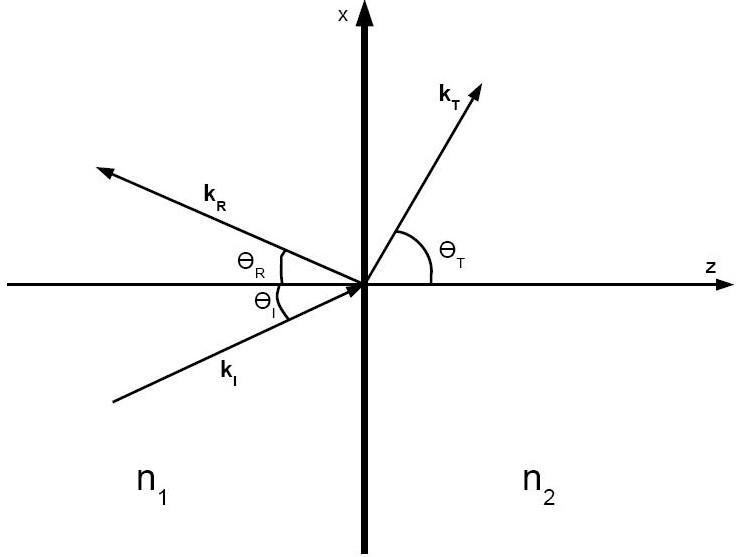
\includegraphics[width = .5\textwidth]{img/TIRDiagram3}
\caption{Light behaviour at media boundary}
\label{criticalangle}
\end{figure}

An important physical consequence can be deduced from this equation: the tangential components of the electric and of the magnetic field cannot be discontinuous at the boundary, so the field is not totally inside the waveguide, but a small part can be found also outside. Indeed, Maxwell's equations impose boundary conditions on the electric and magnetic field, the solution of those equations outside the waveguide cannot transport energy, otherwise the light would not be confined inside the waveguide, the only solution is to have an exponentially decreasing wave called the evanescent wave. This evanescent wave explains why the effective index is present in the formula of the modal propagation costant, the wave, which travels inside the waveguide, propagates inside a medium with fixed refractive index and its tail propagates outside the waveguide where there is a different refractive index. The effective index accounts for this phenomenon.
Evanescent fields are also important when two waveguides are very close to each other: if light travels inside a waveguide and its evanescent tail reaches the neighbouring waveguide the light can penetrate into its core and there is transfer of energy. This allows the coupling of different waveguides or, as we will see later, the coupling between a waveguide and a resonator. It is also interesting to look at the quantum description of this effect: a photon is described by a wave function which is a solution of the Schr{\"o}dinger equation, in the same mathematical way of Maxwell's equations, these impose the continuity of the wavefunction across the medium bondary. If two waveguides are close enough, the wave function is non zero inside both waveguides, so a photon have a non-zero probability to pass through the gap and change waveguide, in quantum mechanics this effect is called quantum tunneling. 
\section{Resonator}
\begin{figure}
\centering
\begin{subfigure}{0.5\textwidth}
\centering
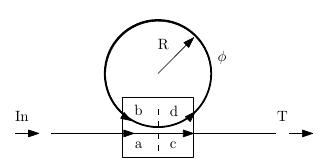
\includegraphics[width = \textwidth]{img/APF}
\caption{}
\end{subfigure}%
\begin{subfigure}{0.5\textwidth}
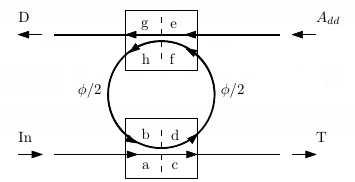
\includegraphics[width = \textwidth]{img/ADF}
\caption{}
\end{subfigure}
\caption{Basic configuration with waveguides and a resonator (a) All Pass Filter (b) Add Drop Filter}\label{basicconfiguration}
\end{figure}

A waveguide can be bent and closed onto itself to provide coherent feedback to the circulating light. This device is called a resonator and it can have different shape, such as a ring or a racetrack. Due to the size of these devices they are called microresonators. For ease of calculation we will treat only microrings with fixed radius. Inside a ring resonator light interferes constructively if the equation $n_{eff} L = m \lambda_m$ is satisfied, where L is the circumference, $m$ is an integer and $\lambda_m$ is the light wavelength. A consequence of constructive interference is that inside the resonator a large amount of energy is stored and the intesity of the field is enhanced. A strong electric field can cause non-linear effects. This is a reason for the importance of resonators: with low power input it is possible to have non-linear effects that usually require a more powerful source. Ring resonators have many applications: for example they can be used as filters for specific wavelengths for multiplexing applications, sensing, signal modulation and active devices for building integrated microlasers.\\
There are two main ways to create circuits with the two basic blocks just described: the first one is a waveguide side coupled to a single ring, and this configuration is called All Pass Filter (APF), while if there are two waveguides coupled to a single ring, the configuration is called Add-Drop Filter (ADF). In figure \ref{basicconfiguration} we can see both configurations. The coupling is possible by means of the evanescent wave, since the gap between the waveguide and the ring is very narrow (on the order of $\simeq 100\, nm$).\\
Coupling can be seen as a quad port beam splitter and the relationship between the complex amplitudes of waves in input and output can be represented with the following matrix
\begin{equation}M = \begin{pmatrix}
r & ik \\
ik & r\\
\end{pmatrix}\end{equation}
where $r$ is the reflection coefficient and $k$ is the transmission coefficient, they satisfy $r^2 +k^2 = 1$. The elements of the matrix can be found by imposing energy conservation among input and output \cite{thesis:masi}. Let us focus now on the APF configuration: using the above matrix we want to find the relation bewteen $a$ and $c$ in order to find the transfer function of the device
\begin{equation}\label{APF}\begin{pmatrix}c \\ d \end{pmatrix} = M \begin{pmatrix}a\\b \end{pmatrix}\end{equation}
$b$ and $d$ are connected with the roundtrip phase condition $b = e^{-\alpha 2\pi R} e^{-i\beta 2\pi R}d \equiv\tau e^{-i\phi(\lambda)}d $, in wich $\alpha$ is the linear absorption coefficient, $R$ the ring radius and $\beta$ is the bent mode wavevector $\beta = \frac{2\pi n_{eff}}{\lambda}$. Solving the system \eqref{APF} leads to the transfer function
\begin{equation}H_{AP} = \frac{c}{a} = \frac{\tau - re^{i\phi(\lambda)}}{r\tau -e^{i\phi(\lambda)}}\end{equation}
for the ADF configuration, the expression of the transfer function can be obtained in a similar way, but now we need to handle two beam splitters, and the round trip phase condition are more complicated: $f = e^{-\alpha \pi R} e^{-i\beta \pi R}d$ and $b=e^{-\alpha \pi R} e^{-i\beta \pi R}h$, working out the calculation we get the final result
\begin{equation}H^D_{AD} = \frac{c}{a} = \frac{k^2\sqrt{\tau} e^{i\phi/2}}{r^2\tau -e^{i\phi}}\qquad H^T_{AD} = \frac{g}{a} = \frac{r(e^{i\phi} - \tau)}{e^{i\phi}-r^2\tau} \end{equation}
Another important quantity is the quality factor $Q = \frac{\lambda}{\Delta \lambda}$, where $\Delta \lambda$ is the full width at half maximum of the lorentzian resonance at wavelength $\lambda$. Equivalently the quality factor can be seen as the ratio between the stored energy inside the cavity and the amount lost per cycle. Furthermore, the quality factor is directly correlated with the enhancement factor $EF$ which is the ratio between the amplitude of the electric field inside the resonator and the exciting electric field. An expression for the quality factor can be obtained by taking two successive resonances and calculating the free spectral range, with a Taylor expansion it can be found \cite{thesis:borghi} for the APF and ADF configurations
\begin{equation}
Q_{APF} = \frac{\pi n_g \lambda_m 2\pi R \sqrt{r\tau}}{(1-r\tau)\lambda_m} \qquad Q_{ADF} = \frac{\pi n_g \lambda_m 2\pi R r\sqrt{\tau}}{(1-r^2\tau)\lambda_m}
\end{equation}
from this equation we can see that it is possible to achieve high quality factor with large rings and low losses. For example with losses in the order of $3 \frac{dB}{\text{cm}}$, a radius of $10\, \mu m$, with an input of $1550$ nm and $3\%$ coupling, the quality factor is approximately $10^4$.
\section{Coupled resonators}\label{coupled}
\begin{figure}[H]
\centering
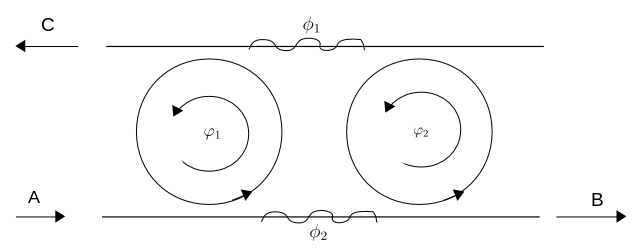
\includegraphics[width = .7\textwidth]{img/coupled}
\caption{Two resonators coupled together}
\label{resonatorcoupled}
\end{figure}
A more interesting configuration of microresonators is presented in figure \ref{resonatorcoupled}. The configuration consists of by two ADF connected in series and it is the configuration on which this work is based. Between the microresonators there is a heater that by heating up the waveguide is able to change the phase of the field travelling inside it. The idea is that in general the generated photons can exit both from T, both from D or one photon in T and one photon in D, but, by changing the phase $\phi_1$ and $\phi_2$, it is possible to decide where the photons exit. A useful quantity that will be needed in this work is the field enhancement of the rings. The analytic expression can be found using the formalism developed in the previous section, and the results are
\[FE_1 = \frac{ie^{i(\varphi_1+\phi_2+\phi_1)}k (e^{i\varphi_2}-r^2\tau_2)-ie^{\frac{i}{2}(\varphi_1+\varphi_2)}k^3(k^2+r^2)\sqrt{\tau_1\tau_2}\tau L^2}{e^{i(\phi_1+\phi_2)}(e^{i\varphi_1}-r^2\tau_1)(e^{i\varphi_2}-r^2\tau_2)-e^{\frac{i}{2}(\varphi_1+\varphi_2)}k^4\sqrt{\tau_1\tau_2}\tau L^2}\]
\[FE_2 = \frac{ie^{i(\varphi_2+\phi_1)}kr (-e^{i\varphi_1}+(r^2+k^2)\tau_1)\tau L}{e^{i(\phi_1+\phi_2)}(e^{i\varphi_1}-r^2\tau_1)(-e^{i\varphi_2}+r^2\tau_2)+e^{\frac{i}{2}(\varphi_1+\varphi_2)}k^4\sqrt{\tau_1\tau_2}\tau L^2}\]
where $FE_1$ refers to the ring on the left and $FE_2$ to the ring on the right, $\varphi = \beta L$ and $L=2\pi R$. Figure \ref{FE} shows field enhancements in the case of $\phi_1 + \phi_2 = 2m\pi$ around the pump wavelength. The condition $\phi_1 + \phi_2 = 2m\pi$ is important because it enhances the optical power inside the ring and, as can be seen from the figure, split the energy equally between the two rings. An equally split energy means that the two rings are indistinguishable and therefore there is the same probability that the photons are generated inside one or the other ring. Indeed, if the energy is not split equally, it means that only one ring works and the configuration is identical to a simple ADF, hence the tuning with the heaters will not work. 


\begin{figure}
\centering
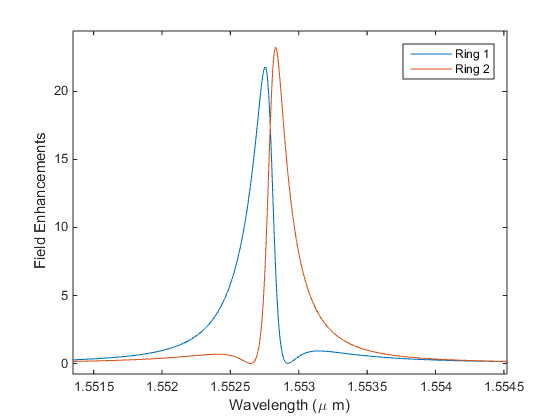
\includegraphics[width = .8\textwidth]{img/FE_fase_2pi}
\caption{Field enhancements with $\phi_1+\phi_2 = 2\pi$, ring 1 refers to the left one and 2 to the right one}
\label{FE}
\end{figure}



\chapter{Physical theory and mathematical model}
\section{Non linear optics}
An electric field inside a medium induce a dipole moment inside the media, the polarization $P$ is defined as the dipole moment per unit volume \cite{book:saleh}. The relation between the polarization and the electric field $E$ is in first approximation linear
\begin{equation}\label{linearP} \mathbf{P} = \varepsilon_0 \chi \mathbf{E}
\end{equation}
where $\varepsilon_0$ is the permittivity of free space and $\chi$ is the eletric susceptibility of the medium which is in general a second rank tensor in order to account for medium anisotropy. If the intensity of the electric field is strong enough, the relation between the field and the polarization is no longer linear and we need to expand the equation \eqref{linearP} in series, in general we find
\begin{equation}\label{nonlinearpolarization}P_i  = \varepsilon_0(\sum_j \chi_{ij}^{(1)} E_j + \sum_{j,k}x_{ijk}^{(2)}E_jE_k + \sum_{j,k,l}\chi_{ijkl}^{(3)}E_jE_kE_l + \dots )\end{equation}
where $\chi^{(i)}$ are tensor of rank $i+1$ and represent the $i$-order susceptibily. This leads to an entire new class of phenomena that have a great interest in photonics, in fact as we'll se later, an electric field with frequency $\omega_1$ can excite a new eletric field with different frequency $\omega_2$. Silicon is a centrosymmetric crystal, this means that if the eletric field change sign, the resulting polarization must change sign equally, hence the even order of susceptibily must vanish, so the first non linear effects of silicon are those of the third order and it's referred as Kerr nonlinearity. For silicon $\chi^{(3)}$ is in the order of $10^{-19} \frac{m^2}{V^2}$ for the real part and $10^{-5} \frac{m^2}{V^2}$ for the imaginary part responsible of the absorption. \\
In order to study non linear phenomena in silicon we take an electric field made up by three waves which propagates along the $z$ direction
\begin{equation}E(z,t) = \sum_{j=1}^{3} \frac{1}{2}(A_j(z)e^{i(\omega_jt -k_jz)}+\text{c.c})\end{equation}
where $k_i = \frac{\omega_i}{c}n$. From the Maxwell equation and the equation \eqref{nonlinearpolarization} is possible to derive the Helmoltz equation
\begin{equation}\label{wavesource}\left(\nabla^2 - \frac{n^2}{c^2}\frac{\partial^2}{\partial t^2}\right)E = \mu_0\frac{\partial^2 P_{NL}}{\partial t^2}\end{equation}
in which there's now a source term on the right hand side of the equation given by the non linear polarization $P_{NL} = \varepsilon_0\chi^{(3)}E^3$. Using the field described above it can be written as
\begin{equation}P_{NL} = \varepsilon_0\chi^{(3)} \sum_{l,j,m=\pm1,\pm2,\pm3}\left(\frac{1}{8}A_lA_jA_l e^{i(\omega_l+\omega_j+\omega_m)t}e^{-i(k_l+k_j+k_m)z}\right)\end{equation}
where it's intended that $\omega_{-j} = -\omega_j$ and $A_{-j} = A^*_j$
from this equation we can see that new frequencies arise, hence the field in equation \eqref{wavesource} is a wave that oscillate with these new frequencies. Different frequencies correspond to different effects, here we focus on Four Wave Mixing terms, for futher reference on other terms see \cite{Leuthold2010}. Four Wave Mixing process arise from the frequency $\omega_n = \omega_l - \omega_j +\omega_m$ that represent also the energy conservation. Futhermore in case of four wave mixing the excited wave satisfy also the satisfies the phase-match conndition $k_n = k_l - k_j + k_m$ as can be seen from the same equation of the energy conserving relation. It's worth to note that every non linear effects have their own phase matching condition, this can be exploited in order to decide which effect we want to study in our device. In fact the efficiency of a process is associated with the phase match parameter \cite{phdthesis:borghi} $\Delta k = k_l - k_j + k_m -k_n$, the maximum efficiency is at $\Delta k = 0$, hence devices can be build in such way that they have the maximum efficiency for one effect and low efficiency for the others. Futhermore if the medium is non dispersive the equation $\Delta k = 0$ is equivalent to the energy conservation relation, in fact $k = \frac{n(\omega)}{c}\omega_k$.\\
\begin{figure}
\centering
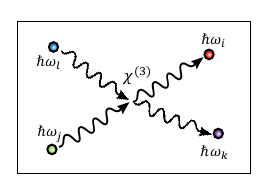
\includegraphics[width = .4\textwidth]{img/FWMphotons}
\caption{Four wave mixing seen as annihilation of two photons and creation of other two photon}
\end{figure}
This classical description however is not suitable for describing photon generation, indeed we need to develop the quantum theory for this phenomena. Four wave mixing in the quantum mechanics point of view can be seen as the annihilation of two photon wich have frequency $\omega_n$ and $\omega_j$ and the simultaneous creation of two photon which have the frequency $\omega_l$ and $\omega_k$. In this scenario the energy conservation is seen as the conservation of photons energy and the phase match condition is the photons momentum conservation.\\
The process used for the generation of photon pairs has $\omega_j = \omega_n \equiv \omega_p$ and it's called non degenerate four wave mixing. The wave with $\omega_p$ has named as pump wave and $\omega_l\equiv \omega_s$ and $\omega_m \equiv \omega_i$ are respectivly the sigNal and idler with the convention that $\omega_s > \omega_i$. In this case the energy conservation can be written as
\begin{equation}\label{conservationenergy}2\omega_p = \omega_s + \omega_i\end{equation}
In the classical derivation the signal stimulate the process and it is necessary for the generation of the idler \cite{phdthesis:borghi}. The classical process, which undergoes this restriction, is called Stimulated Four Wave Mixing. In the quantum description the process become spontaneous, i.e. only the pump field is required for generating the signal and the idler, this process is referred as Spontaneous Four Wave Mixing. The quantum explanation is that the vacuum fluctuation of the electric field provides the necessary stimulus for the process, indeed, in quantum electrodynamics \cite{book:cohen}, the variance of the electric field operator evaluated on the vacuum is finite, even if the mean value of the field is zero.\\
The theory of non liner optics has been discussed here using as principal field the electric field $E$, however for this work is more convenient to take the displacement field $\mathbf{D} = \varepsilon_0\mathbf{E} +\mathbf{P} $ as our fundamental field, this is because in a medium $\mathbf{D}$ is divergenceless. The polarization can be expressed in function of $\mathbf{D}$ as
\begin{equation}P^i = \Gamma^{ij}_1D^j +\Gamma_2^{ijk}D^jD^k + \Gamma_3^{ijkl}D^jD^kD^l + \dots\end{equation}
where the summation over repeated indexes is implicit. Comparing this equation with \eqref{nonlinearpolarization} it's possible to find the relation between the $\Gamma$'s and the $\chi$'s, the relation we are more interested in is
\begin{equation}\Gamma_3^{ijkl} = \frac{\chi_{ijk}^{(3)}}{\varepsilon_0 n^4}\end{equation}
in order to include material dispersion, given the frequency involved, the natural choice is to take
\begin{equation}\Gamma_3^{ijkl} = \frac{\chi_{ijk}^{(3)}}{\varepsilon_0 n^2(\omega_1)n^2(\omega_2)n^2(\omega_3)n^2(\omega_4)}\end{equation}




%H_{NL} = -\frac{1}{3\varepsilon_0}\int\Gamma^{ijkl}_3(\r)D^iD^jD^kD^l\,d\r

\section{Quantum optics}
Since Spontaneous Four Wave Mixing is a quantum phenomenon, a quantum description of light is needed. Standard arguments \cite{book:cohen} leads to the quantization of the electric field, and to the introduction to a light particle: the photon. From a mathematical point of view, the quantization of the electric field is identical to an harmonic oscillator, thus a state with $n$ photons can be writtten with the Dirac's notation as $\Ket{n}$. The displacement field became an operator
\begin{equation}
\mathbf{D}(\r) = \sqrt{\frac{\hbar \omega_k}{2}}a_k \mathbf{D}_k(\r) + \sqrt{\frac{\hbar \omega_k}{2}}a_k^\dagger \mathbf{D}^*_k(\r)
\end{equation}
where $a_k$ is the annihilation operator of a single photon with wavevector $k$, while its adjoint $a_k^\dagger$ is a creation operator and  $\mathbf{D}^*_k(\r)$ is the normalized classical field with wavevector $k$. In this framework the linear Hamiltonian can be written as
\begin{equation}H_L = \int dk \hbar \omega_k a_k^\dagger a_k  \end{equation}
negletting the zero point energy. 





The aim now is to find a correct quantum description for the coherent state of a laser. The photon state number $\Ket{n}$ cannot have the correct classical limit because the expectation value of the electric field on this state vanish no matter how large is the value of $n$. A common way to introduce a coherent state is to find the eigenstates of the annihilation operator:
\begin{equation}\label{eigenvalue}
a_k\ket{\alpha} = \alpha \ket{\alpha}
\end{equation}
where $\alpha$ can be a complex number. We can express this state as a sum of the number states $\ket{n}$, since they form a complete set:
\begin{equation}\ket{\alpha} = \sum_{n=0}^{+\infty} C_n \ket{n}\end{equation}
equation \eqref{eigenvalue} becomes
\begin{equation}a_k\sum_{n=0}^{+\infty} C_n \ket{n} = \sum_{n=0}^{+\infty} C_n\sqrt{n}\ket{n-1} =\alpha\sum_{n=0}^{+\infty} C_n \ket{n}\end{equation}
equation coefficients of $\ket{n}$ on both sides leads to
\begin{equation}C_n = \frac{\alpha}{\sqrt{n}}C_{n-1} = \frac{\alpha^2}{\sqrt{n(n-1)}} = \dots = \frac{\alpha^n}{\sqrt{n!}}C_0\end{equation}
using the fact that the state must be normalized $\Braket{\alpha|\alpha} = 1$ is possible to determine $C_0$ and in conclusion the coherent state can be written as
\begin{equation}\label{coherentstate}
\ket{\alpha} = e^{-\frac{1}{2}|\alpha|^2}\sum_{n=0}^{+\infty} \frac{\alpha^n}{\sqrt{n!}}\ket{n}
\end{equation}
to find a physical meaning of $\alpha$ we can evaluate the expectation value of the photon number operator $\hat{n} = a_k^\dagger a_k$:
\begin{equation}\braket{\alpha|\hat{n}|\alpha} = |\alpha|^2 \end{equation}
hence $|\alpha|^2$ is the avarege photon number of the field. The coherent states $\ket{\alpha}$ are used to represent a classical state, this is due to several reasons which are
\begin{enumerate}[(i)]
\item the expectation value of the electric field is a classical field
\item the fluctuations of the electric field is the same as for the vacuum
\item the states become well localized in phase with increasing of the photon number
\end{enumerate}
an equivalent way to obtain a coherent state $\ket{\alpha}$ is to use the displacement operator defined as 
\begin{equation}\label{def:displacement}\hat{D}(\alpha) = e^{\alpha a_k^\dagger -\text{H.c}}\end{equation}
this operator applied on the vacumm generate exaclty $\ket{\alpha}$, in fact, using the Baker-Campbell-Hausdorff formula, the exponential can be written as:
\begin{equation}\hat{D}(\alpha) = e^{-\frac{1}{2}|\alpha|^2}e^{\alpha a_k^\dagger} e^{-\alpha^* a_k}\end{equation}
when it acts on the vacuum the exponential with the annihilation operators does nothing, so the second exponential can be expanded in Taylor's series:
\begin{equation}\hat{D}(\alpha)\ket{vac} = e^{-\frac{1}{2}|\alpha|^2}\sum_{n=0}^{+\infty}\frac{(\alpha a_k^\dagger)^n}{n!}\ket{vac} = e^{-\frac{1}{2}|\alpha|^2}\sum_{n=0}^{+\infty} \frac{\alpha^n}{\sqrt{n!}}\ket{n}  \end{equation}
exaclty what we found in equation \eqref{coherentstate}.\\
This treatment only describes states where all photons have the same wavevector $k$, but it is simple to generalize the displacement operator in order to generate state with photons with different wavevectors. We can write the displacement operator as
\begin{equation}\hat{D}(\alpha) = e^{\alpha A^\dagger_P -\text{H.c}}\end{equation}
where $A^\dagger_P = \int dk \phi_P(k) a_k^\dagger$ where $|\phi(k)|^2$ is the probability of finding a photon with wavevector $k$ and it is normalized according to $\int dk |\phi_P(k)|^2 = 1$.


\section{Asymptotic field treatment}\label{section:asymptotic}
\begin{figure}
\centering
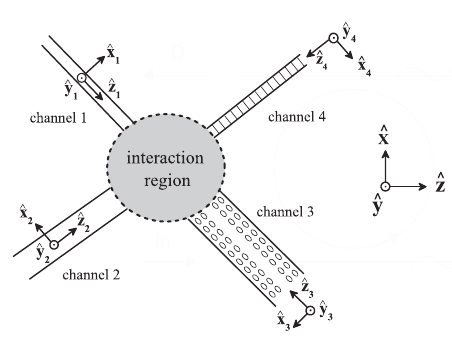
\includegraphics[width = .7\textwidth]{img/asymptotic}
\caption{General structure of interest, the channels can be of different types and non linearities are confined in the interaction region}
\label{generalstructure}
\end{figure}



Most of this section is developed in \cite{Liscidini2012}, here i summarize the key point needed for the next chapter and ease the treatment to single mode field.\\ The idea behind this theory is to provide a easier way to study complex stuctures sketched in figure \ref{generalstructure}. The strategy is borrowed from the theory of scattering in quantum mechanics, an asympotitic-in ad an asymptotic-out state are introduces corresponding to an incident wave packet at $t = -\infty$ and an outgoing wavepacket at $t = +\infty$. The relation between these two state consitutes a solution of the scattering problem itself. Let's consider the general structure in figure \ref{generalstructure}, the first assumption is that the incoming energy can reach the interaction region, where the non linear effects arise, only through the channels. The coordinates of the channels are labelled as $\r_n = (x_n,y_n,z_n)$ where $n$ identifies the channel and the $z_n$-axis point toward the interaction region and the origin $z_n = 0$ is near the center of the interaction region. The starting point is the introduction of the mode field $\mathbf{D}_{n,k}(\r_n)$ for every channels, hence the total field in the set of channels is:
\begin{equation}\mathbf{D}(\r,t) = \sum_n\int_{-\infty}^{+\infty}dk \gamma_{n,k} e^{-i\omega_{n,k}t}\mathbf{D}_{n,k}(\r)  + \text{c.c}\end{equation}
clearly $\mathbf{D}_{n,-k}$ is not indipendent from $\mathbf{D}_{n,k}$ and the relation can be fixed by taking
\begin{equation}\label{ddstar}\mathbf{D}_{n,-k} = \mathbf{D}*_{n,k}\end{equation}

Now we look for solutions of the Maxwell's equations for the structure that have frequency $\omega_{n,k}$ with positive $k$ and have the mode field of the form
\begin{equation}\mathbf{D}^{asy-in}_{n,k} =\mathbf{D}_{n,k}(\r_n) + \mathbf{D}^{out}_{n,k}\end{equation}
where far from the interaction region $\mathbf{D}^{out}_{n,k}$ represent a outgoing wave in each channel, that is
\begin{equation}\label{asyin}\mathbf{D}^{asy-in}_{n,k} \sim \mathbf{D}_{n,k}(\r_n) + \sum_{n'}\int_{0}^{+\infty}dk' T^{out}_{n,n'}(k,k')\mathbf{D}_{n',-k'}(r_{n'})\end{equation}
where $\mathbf{D}^{asy-in}_{n,k}$ is called asymptotic-in mode field and far from the interaction region it corresponds to a wave incoming in channel $n$ and outgoing waves in every channel. % If we construct a superposition of asymptotic-in mode fields
%\begin{equation}\mathbf{D}(\r) = \sum_n \int_0^{+\infty}dk \alpha_{n,k}e^{-i\omega_{n,k}t} \mathbf{D}^{asy-in}_{n,k} + \text{c.c}\end{equation}
%where we choose $\alpha_{n,k}$ such that for $k>0$ $ \gamma_{n,k} = \alpha_{n,k}$
Similarly asymptotic-out mode field is introduces as full solution of Maxwell equation with positive $k$ and of the form
\begin{equation}\mathbf{D}^{asy-out}_{n,k} =\mathbf{D}_{n,-k}(\r_n) + \mathbf{D}^{in}_{n,k}\end{equation}
where $\mathbf{D}^{in}_{n,k}$ far from the interaction region consist of incoming waves in each channel, i.e.
\begin{equation}\label{asyout}\mathbf{D}^{asy-out}_{n,k} \sim \mathbf{D}_{n,-k}(\r_n) + \sum_{n'}\int_{0}^{+\infty}dk' T^{in}_{n,n'}(k,k')\mathbf{D}_{n',k'}(r_{n'})\end{equation} 
Just like in \eqref{ddstar} asymptotic-out field and asymptotic-in field are not indipendent, but comparing \eqref{asyin} and \eqref{asyout} we find
\begin{equation}\mathbf{D}^{asy-out}_{n,k}(\r) = [\mathbf{D}^{asy-in}_{n,k}(\r)]^*\end{equation}
The final step is to quantize the electric field 
\begin{equation}\mathbf{D}(\r) = \sum_n \int_{-\infty}^{+\infty}dk \sqrt{\frac{\hbar \omega_{n,k}}{2}}c_{n,k}\mathbf{D}_{n,k}(\r) + \text{H.c}\end{equation}
the operators $c_{n,k}$ and their adjoint $c_{n,k}^\dagger$ satisfy the canonical commutation
\begin{equation}[c_{n,k},c_{n',k'}] = 0 \qquad [c_{n,k},c_{n',k'}^\dagger] = \delta_{nn'}\delta(k-k')\end{equation}
We can write the field operator as a superposition of asymptotic-in fields
\begin{equation}\label{dasyin}\mathbf{D}(\r) = \sum_n \int_{0}^{+\infty}dk \sqrt{\frac{\hbar \omega_{n,k}}{2}}a_{n,k}\mathbf{D}_{n,k}^{asy-in}(\r) + \text{H.c}\end{equation}
where again the operators $a_{n,k}$ satisfy
\begin{equation}\label{acommutator}[a_{n,k},a_{n',k'}] = 0 \qquad [a_{n,k},a_{n',k'}^\dagger] = \delta_{nn'}\delta(k-k')\end{equation}
or we can also write the field operator as a superposition of asymptotic-out fields
\begin{equation}\label{dasyout}\mathbf{D}(\r) = \sum_n \int_{0}^{+\infty}dk \sqrt{\frac{\hbar \omega_{n,k}}{2}}b_{n,k}\mathbf{D}_{n,k}^{asy-out}(\r) + \text{H.c}\end{equation}
where again
\begin{equation}[b_{n,k},b_{n',k'}] = 0 \qquad [b_{n,k},b_{n',k'}^\dagger] = \delta_{nn'}\delta(k-k')\end{equation}
the utility of this approch is that the linear Hamiltonian can be written with the state of the whole structure, not only the state of rings and waveguides, hence the linear Hamiltonian is diagonal. The full Hamiltonian is therefore the sum of a diagonal term (the linear one) and a non diagonal term (non linear term).

\section{Backward Heisenberg picture approach}\label{heinsemberg}
Assuming the knowledge of the Hamiltonian of the system, this section is devoted on the formalism used to solve the scattering problem subject to the Hamiltonian of the form $H = H_L +H_{NL}$ where $H_L$ is the linear Hamiltonian and $H_{NL}$ is the non linear part. Instead of working in the Schr{\"o}dinger picture it is easier to work in the Heinsenberg picture. 
We want to study what happens to a initial state $\ket{\psi(t_0)}$, $t_0\ll 0$ incident to a interaction region with nonlinearities and find the final state $\ket{\psi(t_1)}$, $t_1\gg 0$. The dynamics is given by the full Hamiltonian $H$
\begin{equation}\label{evolution}\ket{\psi(t_1)} = e^{-\frac{i}{\hbar}H (t_1-t_0)}\ket{\psi(t_0)}\end{equation}
Let's take the assumption that the non linear interactions happens at $t=0$ and we takes $t_0 \to -\infty$ and $t_1 \to -\infty$ such that the initial and final states are far from the interaction region. We can define an asymptotic-in state $\ket{\psi_{in}}$ as the state at $t=0$ to whom $\ket{\psi(t_0)}$ would evolve if the evolution occurs only with $H_L$, that is
\begin{equation}\label{statein}\ket{\psi_{in}} = e^{-\frac{i}{\hbar}H_L (0-t_0)}\ket{\psi(t_0)} = e^{\frac{i}{\hbar}H_Lt_0}\ket{\psi(t_0)}\end{equation}
and similarly we can define the asymptotic-out state $\ket{\psi_{out}}$ as the state at $t=0$ that would evolve into $\ket{\psi(t_1)}$ if the evolution is dictated by $H_L$, that is
\begin{equation}\ket{\psi(t_1)} = e^{-\frac{i}{\hbar}H_L t_1}\ket{\psi_{out}}\end{equation}
using equation \eqref{evolution} and \eqref{statein} inside the last equation we can find the relation between the asymptotic-in state and the asyptotic-out

\begin{equation}
\begin{split}
e^{-\frac{i}{\hbar}H (t_1-t_0)}\ket{\psi(t_0)} = e^{-\frac{i}{\hbar}H_L t_1}\ket{\psi_{out}} \\
e^{-\frac{i}{\hbar}H (t_1-t_0)}e^{-\frac{i}{\hbar}H_Lt_0}\ket{\psi_{in}} = e^{-\frac{i}{\hbar}H_L t_1}\ket{\psi_{out}}
\end{split}
\end{equation}
and finally
\begin{equation}\label{relation:inout}\ket{\psi_{out}} = U(t_1,t_0) \ket{\psi_{in}}\end{equation}
where 
\begin{equation}\label{U}
U(t',t) = e^{\frac{i}{\hbar}H_Lt'}e^{-\frac{i}{\hbar}H(t'-t)}e^{-\frac{i}{\hbar}H_Lt}
\end{equation}
the advantage of this approch is that the non linear scattering problem is contained only in the transition $\ket{\psi_{in}} \to \ket{\psi_{out}}$ and it's easy to calculate the asymptotic states since they are a linear evolution of initial and final state. Hence if we start from $\ket{\psi(t_0)}$ we can easly calculate $\ket{\psi_{in}}$, then we solve the non linear problem in the transition $\ket{\psi_{in}} \to \ket{\psi_{out}}$ and finally we can easly determine the final state $\ket{\psi(t_1)}$. For this reason now we study the dynamics of $U(t_1,t_0)$, differentiating equation \eqref{U} we obtain
\begin{equation}\label{dynamicU}-i\hbar \frac{\partial U(t',t)}{\partial t} = U(t',t)V(t)\end{equation}
where $V(t)$ has been defined as
\begin{equation}V(t) \equiv  e^{\frac{i}{\hbar}H_Lt}H_{NL}e^{-\frac{i}{\hbar}H_Lt} \equiv U_L^\dagger H_{NL} U_L\end{equation}
let's consider an asymptotic-in state of the form 
\begin{equation}\ket{\psi_{in}} = e^O \ket{vac}\end{equation}
where $O$ is a Schr{\"o}dinger operator. With this definition we have in mind the displacement operator defined in \eqref{def:displacement} that generates the coherent state of the laser. From equation \eqref{relation:inout} we can write
\begin{equation}\label{outfinal}\ket{\psi_{out}} = U(t_1,t_0)e^O \ket{vac}\end{equation}
using the fact that both $H$ and $H_L$ have at least one lowering operator on the right we can say $H\ket{vac} = H_L\ket{vac} = 0$, therefore also
\begin{equation}U(t_1,t_0)\ket{vac}= U^\dagger(t_1,t_0)\ket{vac}= \ket{vac}\end{equation}
this proprierty allows us to write
\begin{equation}\ket{\psi_{out}} = U(t_1,t_0)e^OU^\dagger(t_1,t_0)\ket{vac} = e^{U(t_1,t_0)OU^\dagger(t_1,t_0) }\ket{vac}\equiv e^{\overline{O}(t_0)}\ket{vac}\end{equation}
where 
\begin{equation}\label{dynamicO}\overline{O}(t) = U(t_1,t)OU^\dagger(t_1,t)\end{equation}
and it satisfies $\overline{O}(t_1) = O$. Differentiating \eqref{dynamicO} and using \eqref{dynamicU} we find
\begin{equation}\label{motionO}i\hbar \frac{d\overline{O}(t)}{dt} = [\overline{O}(t),\hat{V}(t)]\end{equation}
where
\begin{equation}\hat{V}(t) \equiv U(t_1,t)V(t)U^\dagger(t_1,t)\end{equation}
In conclusion the approch that can be taken is first find $V(t)$ and $\hat{V}(t)$ for the system and then integrate equation \eqref{motionO} from $t=t_1$ back to $t=t_0$ subjet to the final condition $\overline{O}(t_1) = O$, after that we can determine $\ket{\psi_{out}}$ using \eqref{outfinal}.

\chapter{Photons generation in coupled resonators}
\begin{figure}[H]
\centering
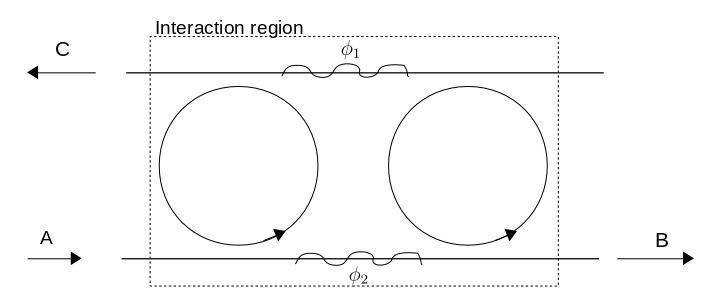
\includegraphics[width = .8\textwidth]{img/system}
\caption{Coupled resonators, Spontaneous Four wave mixing happens only inside the rings, there are three channels labelled as A,B and C}
\label{couplesstructure}
\end{figure}

In this last chapter we study the generation of entangled photons via Spontaneous Four Wave Mixing in the structure of figure \ref{couplesstructure}. As can be seen from the figure, the structure is composed by two ADF in series, the channel are labelled with the lettera $A$, $B$, $C$ and $D$, in this work we assume that the input is in the channel $A$ and the output can be in either in $B$ or in $C$. The work starts by writing the non linear Hamiltonian in terms of the asymptotic states developed in section \ref{section:asymptotic}, then we solve the dynamics of the photons state using the backward Heisenberg approch developed in section \ref{heinsemberg} and finally we study the results.
\section{Asymptotic fields}
\begin{figure}[H]
\centering
\begin{subfigure}{0.5\textwidth}
\centering
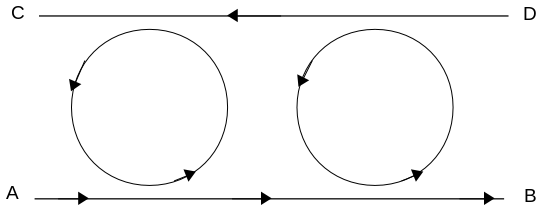
\includegraphics[width = \textwidth]{img/Asyina}
\caption{Asymptotic in field for channel $A$}
\end{subfigure}%
\begin{subfigure}{0.5\textwidth}
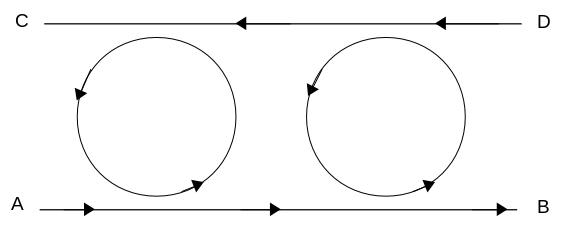
\includegraphics[width = \textwidth]{img/Asyoutb}
\caption{Asymptotic out field for channel $B$}
\end{subfigure}
\caption{Asymptotic fields for the coupled resonators, the ring on the left is identified as 1, while the ring on the right as 2}\label{asyfields}
\end{figure}
We take as input state a coherent state in channel A, so we can write it as $\ket{\psi_{in}} = e^{\alpha A_p^\dagger - \text{H.c}}\ket{vac}$ where $A_p^\dagger = \int dk \phi_P(k) a_k^\dagger$. The non linear Hamiltonian is \cite{Sipe2004}
\begin{equation}\label{nonlinearhamiltonian}H_{NL} = -\frac{1}{3\varepsilon_0}\int\Gamma^{ijkl}_3(\r)D^iD^jD^kD^l\,d\r\end{equation}
where the summation over repeated indexes is implicit. Since the asymptotic states are a complete basis we can expand $D$ either on the asympotic-out states, or on the asymptotic-in, we can chose to expand two field of \eqref{nonlinearhamiltonian} in terms of the asymptotic-in and the other two in terms of the asympotic-in.
Keeping only the Spontaneous Four Wave Mixing terms we arrive at:
\begin{multline}H_{NL} = -\int dk_1dk_2dk_3dk_4S_{bb}(k_1,k_2,k_3,k_4)a_{k_1}a_{k_2}b_{b,k_3}^\dagger b_{b,k_4}^\dagger \\-2\int dk_1dk_2dk_3dk_4S_{bc}(k_1,k_2,k_3,k_4)a_{k_1}a_{k_2}b_{b,k_3}^\dagger b_{c,k_4}^\dagger\\ -\int dk_1dk_2dk_3dk_4S_{cc}(k_1,k_2,k_3,k_4)a_{k_1}a_{k_2}b_{c,k_3}^\dagger b_{c,k_4}^\dagger +\text{H.c.}\end{multline}
where where $a_k$ is the annihilation operator associated with channel A, $b_{b,k}$ is for channel B and $b_{c,k}$ refers to channel C and we defined the following quantity
\begin{multline}\label{S}
S_{xy}(k_1,k_2,k_3,k_4) = \frac{3}{2\varepsilon_0}\sqrt{\frac{(\hbar\omega_{k_1})(\hbar\omega_{k_2})(\hbar\omega_{k_3})(\hbar\omega_{k_4})}{16}}\cdot \\ \int d\r \Gamma^{ijkl}_3D^{i,asy-in}_{a,k_1}(\r)D^{j,asy-in}_{a,k_2}(\r)\left[D^{k,asy-out}_{x,k_3}(\r)\right]^*\left[D^{l,asy-out}_{y,k_4}(\r)\right]^*
\end{multline}
we derive now the explicit form of $S_{bb}$ and in analogy also for $S_{bc}$ and $S_{cc}$. In section \ref{section:asymptotic} we stated that the asympotic-in field associated with channel $A$ corresponds to a wave incoming in channel $A$ and outgoing waves in every channel, and similarly asymptotic-out field of channel $B$ consist of an outgoing wave in channel $B$ and incoming waves in the other channels. These asympotitic fields are depicted in figure \ref{asyfields}. The integral of $S_{bb}$ is performed in general over all the space, but outside waveguides and resonators the field is zero, futhermore, since the field inside the ring in enhanced with respect to the field in the waveguide, we can neglet the contribution of the field in the waveguides. Therefore the integration can be performed only over the rings. With this assumption we can write the asymptotic fields as
\begin{equation}\mathbf{D}^{asy-in\,(rings)}_{a,k} = FE_{1a}(\omega) \mathbf{d}^1_{k_1}(\r_\perp)e^{ik_1z} + FE_{2a}(\omega) \mathbf{d}_{k_2}^2(\r_\perp)e^{ik_2z} \end{equation}
where $z$ is the coordinate in the counterclockwise direction along the rings circunference and $\r_\perp$ are the coordinates perpendicular to $z$. $FE_{1a}$ is the field enhancement of the first ring when the input wave is in channel $A$, while obviously $FE_{2a}$ refers to the second ring. $\mathbf{d}^1_{k_1}(\r_\perp)$ is the linear mode profile. Similarly the asymptotic-out field associated with channel $B$ can be written as
\begin{equation}\mathbf{D}^{asy-out\,(rings)}_{b,k} = FE_{1b}(\omega) \mathbf{d}^1_{k_1}(\r_\perp)e^{ik_1z} + FE_{2b}(\omega)\mathbf{d}_{k_2}^2(\r_\perp)e^{ik_2z} \end{equation}
using the last two equations in \eqref{S} leads to a lot of terms, everyone associated with a specific physical interpretation. In particular every terms correspond to a possible path for the photons that are scattered in the channel $B$, for example, the annihilated pump photons can be both inside the first ring, or both in the second one or even one in the first ring, one in the second one. Same argument for the created photons that can be created both inside the first ring, both inside the second or one in each ring. The combination of these paths are represented by all terms in $S_{bb}$, however each of this terms are proportional to the field $\mathbf{d}^1_{k_1}(\r_{\perp})$ and $\mathbf{d}^2_{k_2}(\r_{\perp})$ that are non zero only inside the ring, therefore a term that contain a factor $\mathbf{d}^2_{k_2}(\r_{\perp})\mathbf{d}^2_{k_2}(\r_{\perp})$ is zero everywhere, because in the first ring the second factor is zero and in the second ring the first factor is zero. The only term that survive the integration are those who have all factors equal to  $\mathbf{d}^2_{k_2}(\r_{\perp})$ or $\mathbf{d}^2_{k_2}(\r_{\perp})$, that is only the path where the two pump photons are annihilated in the same ring where the signal and indler photons are created. Therefore we can write $S_{bb}$ as
\begin{multline}S_{bb} =\frac{3}{2\varepsilon_0}\sqrt{\frac{(\hbar\omega_{k_1})(\hbar\omega_{k_2})(\hbar\omega_{k_3})(\hbar\omega_{k_4})}{16}}\Bigg( \\ \int d\r \Gamma^{ijkl}_3FE_{1a}(\omega_1)FE_{1a}(\omega_2)FE^*_{1b}(\omega_3)FE^*_{1b}(\omega_4)d^{1,i}_{k_1}(\r_{\perp})d^{1,j}_{k_2}(\r_{\perp})d^{1,k}_{k_3}(\r_{\perp})d^{1,l}_{k_4}(\r_{\perp})e^{i\Delta k z} +\\
\int d\r \Gamma^{ijkl}_3FE_{2a}(\omega_1)FE_{2a}(\omega_2)FE^*_{2b}(\omega_3)FE^*_{2b}(\omega_4)d^{2,i}_{k_1}(\r_{\perp})d^{2,j}_{k_2}(\r_{\perp})d^{2,k}_{k_3}(\r_{\perp})d^{2,l}_{k_4}(\r_{\perp})e^{i\Delta k z}\Bigg)\end{multline}
where $\Delta k = k_1 + k_2 -k_3 - k_4$. The integration in $z$ can be done easly
\begin{equation}\int_0^{L} e^{i\Delta k z} dz = \frac{1}{i\Delta k}(e^{i\Delta k L} - 1) = \frac{e^{i\Delta k L/2}}{i\Delta k}(e^{i\Delta k L/2}- e^{-i\Delta k L/2}) = \frac{2}{\Delta k}e^{i\Delta k L/2} \sin\left(\Delta k \frac{L}{2}\right)\end{equation}
which can be written as $\frac{L}{\pi}e^{i\Delta k L/2} \text{sinc}\left(\Delta k \frac{L}{2\pi}\right)$. If we define the following
\begin{equation}\gamma_1 = \frac{3}{2\varepsilon_0}\int d\r_\perp \Gamma^{ijkl}_3d^{1,i}_{k_1}(\r_{\perp})d^{1,j}_{k_2}(\r_{\perp})d^{1,k}_{k_3}(\r_{\perp})d^{1,l}_{k_4}(\r_{\perp})\end{equation}
and the related $\gamma_2$, the expression for $S_{bb}$ is finally:
\begin{multline}\label{sbbfinal} S_{bb} = \frac{L}{\pi}e^{i\Delta k L/2} \text{sinc}\left(\Delta k \frac{L}{2\pi}\right) \sqrt{\frac{(\hbar\omega_{k_1})(\hbar\omega_{k_2})(\hbar\omega_{k_3})(\hbar\omega_{k_4})}{16}}\Bigg(\\ \gamma_1 FE_{1a}(\omega_1)FE_{1a}(\omega_2)FE^*_{1b}(\omega_3)FE^*_{1b}(\omega_4) +\gamma_2 FE_{2a}(\omega_1)FE_{2a}(\omega_2)FE^*_{2b}(\omega_3)FE^*_{2b}(\omega_4)\Bigg)\end{multline}




\section{Output state}
With this expression in hands we can switch to the Heisenberg picture e we can define
\begin{equation}\label{potential}
V(t) = U_L^\dagger H_{NL}U_{L}\end{equation}
since the operator $U_L$ satisfies the unitary relation $U_L U_L^\dagger = U_L^\dagger U_L = \mathbbm{1}$ we can isert $U_L^\dagger U_L$ between every annhilation and creation operators and define the time dependent operators, for example $a_{k}(t) \equiv U_L^\dagger a_{k}U_L$. Time dependent operators satisfies the Heisenberg equation
\begin{equation}\frac{da_{k}}{dt} = \frac{1}{i\hbar}[a_{k},H_L]\end{equation}
which we can solve for every operators. For example for $a_{k}$ the commutator with the linear Hamiltonian is:
\begin{equation}[a_{k},H_L] = \int dk'\hbar \omega_{k'}a_{k} a_{k'}^\dagger a_{k'}-\int dk'\hbar \omega_{k'}a_{k'}^\dagger a_{k'}a_{k}\end{equation}
we know that $[a_k,a_{k'}^\dagger] = \delta(k-k')\implies a_{k} a_{k'}^\dagger = \delta(k-k') + a_{k'}^\dagger a_{k}$ substituting this into the first term we arrive at
\begin{equation}[a_{k},H_L] = \int dk'\hbar \omega_{k'}a_{k}\delta(k-k') = \hbar \omega_{k}a_{k}\end{equation}
so the Heisenberg equation can be written as
\begin{equation}\frac{da_{k}}{dt} = -i\omega_{k}a_{k}\end{equation}
which has the trivial solution $a_k(t) = a_k(0)e^{-i\omega_k t}$, since $a_k(0) = a_k$ we can write \eqref{potential} 
\begin{equation}V(t) = V_{bb} + 2V_{bc} + V_{cc}\end{equation}
where
\begin{equation}V_{xy} = -\int dk_1dk_2dk_3dk_4S_{xy}(k_1,k_2,k_3,k_4;t)a_{k_1}a_{k_2}b_{x,k_3}^\dagger b_{y,k_4}^\dagger +\text{H.c} \end{equation}
and $S_{xy}(k_1,k_2,k_3,k_4;t) = S_{xy}(k_1,k_2,k_3,k_4)e^{-i(\omega_{k1}+\omega_{k2}-\omega_{k3}-\omega_{k4})t}$. In a similar way it's possible to construct $\hat{V}(t)$
\begin{equation}\hat{V}(t) = U(t_1,t)V(t)U^\dagger(t_1,t) = \hat{V}_{bb}(t) + 2\hat{V}_{bc}(t) + \hat{V}_{cc}(t)\end{equation}
where 
\begin{equation}\hat{V}_{xy}(t) = -\int dk_1dk_2dk_3dk_4S_{xy}(k_1,k_2,k_3,k_4;t)\overline{a}_{k_1}(t)\overline{a}_{k_2}(t)\overline{b}_{x,k_3}^\dagger(t) \overline{b}_{y,k_4}^\dagger(t) +\text{H.c}\end{equation}
now we have all the elements for integrating the equation \eqref{dynamicO}, we need to solve it for the operator $\overline{a}^\dagger_{k}(t)$
\begin{equation}\label{meinkampf}-i\hbar \frac{d\overline{a}^\dagger_{k}(t)}{dt} = [\overline{a}^\dagger_{k},\hat{V}(t)] = [\overline{a}^\dagger_{k},\hat{V}_{bb}(t)] + [\overline{a}^\dagger_{k},2\hat{V}_{bc}(t)] +[\overline{a}^\dagger_{k},\hat{V}_{cc}(t)]\end{equation}
we need to work out the three commutator, they are all  similar, so we show only one
\begin{multline}[\overline{a}^\dagger_{k},\hat{V}_{bb}(t)] = -\int dk_1dk_2dk_3dk_4S_{bb}(k_1,k_2,k_3,k_4;t)\overline{a}^\dagger_{k}(t)\overline{a}_{k_1}(t)\overline{a}_{k_2}(t)\overline{b}_{b,k_3}^\dagger(t) \overline{b}_{b,k_4}^\dagger(t) \\
-\int dk_1dk_2dk_3dk_4S_{bb}(k_1,k_2,k_3,k_4;t)\overline{a}^\dagger_{k}(t)\overline{a}^\dagger_{k_1}(t)\overline{a}^\dagger_{k_2}(t)\overline{b}_{b,k_3}(t) \overline{b}_{b,k_4}(t) \\
+ \int dk_1dk_2dk_3dk_4S_{bb}(k_1,k_2,k_3,k_4;t)\overline{a}_{k_1}(t)\overline{a}_{k_2}(t)\overline{b}_{b,k_3}^\dagger(t) \overline{b}_{b,k_4}^\dagger(t)\overline{a}^\dagger_{k}(t)\\ 
+ \int dk_1dk_2dk_3dk_4S_{bb}(k_1,k_2,k_3,k{}_4;t)\overline{a}^\dagger_{k}(t)\overline{a}^\dagger_{k_1}(t)\overline{a}^\dagger_{k_2}(t)\overline{b}_{b,k_3}(t) \overline{b}_{b,k_4}\overline{a}^\dagger_{k}(t) \end{multline}
the second and the fourth term are indentical, therefore they can be eliminated, for the first one we can use \eqref{acommutator}, at the end we get
\begin{equation}[\overline{a}^\dagger_{k},\hat{V}_{bb}(t)] = 2\int dk_1 dk_2 dk_3 S_{bb}(k_1,k_2,k_3,k,t)\overline{a}_{k_1}(t)\overline{b}_{b,k_2}^\dagger(t)\overline{b}_{b,k_3}^\dagger(t)\end{equation}
the zeroth-order solution of \eqref{meinkampf} is $\overline{a}^\dagger_{k}(t) = \overline{a}^\dagger_{k}(t_1) = a_k^\dagger$, so, the first order solution is
\begin{multline}\label{abarra}\overline{a}^\dagger_{k}(t) = a_k^\dagger + \frac{2}{i\hbar}\int dk_1dk_2 dk_3 \int_{t_1}^tS_{bb}(k_1,k_2,k_3,k,t)a_{k_1}b_{b,k_2}^\dagger b_{b,k_3}^\dagger \\+\frac{4}{i\hbar}\int dk_1dk_2 dk_3 \int_{t_1}^tS_{bc}(k_1,k_2,k_3,k,t)a_{k_1}b_{b,k_2}^\dagger b_{c,k_3}^\dagger \\
+ \frac{2}{i\hbar}\int dk_1dk_2 dk_3 \int_{t_1}^tS_{cc}(k_1,k_2,k_3,k,t)a_{k_1}b_{c,k_2}^\dagger b_{c,k_3}^\dagger \end{multline}
with this expression we can write the output state as
\begin{equation}\ket{\psi_{out}} = e^{\alpha \overline{A}_P^\dagger(t_0)-\text{H.c}}\end{equation}
where $\overline{A}_P^\dagger(t_0) = \int dk \phi_P(k)\overline{a}_k^\dagger(t_0)$. Now we take $t_0\to -\infty$ and $t_1 \to +\infty$ and we integrate in time using $\frac{1}{2\pi} \int dt e^{i\omega t} = \delta(\omega)$, so we can write, for example, the second term of \eqref{abarra} as
\begin{equation}\frac{2i2\pi }{\hbar}\int dk_1dk_2 dk_3S_{bb}(k_1,k_2,k_3,k)\delta(\omega_{k}+\omega_{k1}-\omega_{k2}-\omega_{k3})a_{k_1}b_{b,k_2}^\dagger b_{b,k_3}^\dagger \end{equation}
we can use now the Baker-Campbell-Hausdorff formula to expand $\ket{\psi_{out}}$, the formula states $e^{A+B} = e^{A}e^{-\frac{1}{2}[A,B]} e^{B}$, we take 
\begin{equation}A =\alpha \int dk \phi_P(k)a_k^\dagger - \text{H.c} \end{equation}
\begin{equation}B = \frac{2i2\pi }{\hbar}\int dk dk_1dk_2 dk_3\phi_P(k)S_{bb}(k_1,k_2,k_3,k)\delta(\omega_{k}+\omega_{k1}-\omega_{k2}-\omega_{k3})a_{k_1}b_{b,k_2}^\dagger b_{b,k_3}^\dagger -\text{H.c} +\dots\end{equation}
plus the other terms related to $bc$ and $cc$, we need to work out the commutator, again using \eqref{acommutator}, we obtain
\begin{equation}-\frac{1}{2}[A,B] = \frac{2\pi i \alpha^2}{\hbar}\int dk dk_1dk_2 dk_3\phi_P(k)\phi_P(k_1)S_{bb}(k_1,k_2,k_3,k)\delta(\omega_{k}+\omega_{k1}-\omega_{k2}-\omega_{k3})b_{b,k_2}^\dagger b_{b,k_3}^\dagger -\text{H.c} +\dots\end{equation}
where we negleted all non two photon creation operator terms and the dots still refer to $bc$ and $cc$. We can notice that $e^B\ket{vac} = \ket{vac}$, so we can write the final state as
\begin{equation}\ket{\psi_{out}} = e^{\alpha A_P^\dagger + \beta_{bb} C^\dagger_{II\,bb}+ 2\beta_{bc} C^\dagger_{II\,bc}+ \beta_{cc} C^\dagger_{II\,cc}-\text{H.c}}\ket{vac}\end{equation}
where
\begin{equation}C^\dagger_{II\, xy} = \frac{1}{\sqrt{2}}\int dk_1 dk_2 \phi_{xy}(k_1,k_2)b_{x,k_1}^\dagger b_{y,k_2}^\dagger \end{equation}
and $\phi_{xy}(k_1,k_2)$ is the biphoton wave function 
\begin{equation}\label{biphoton}\phi_{xy}(k_1,k_2) = \frac{2\pi i \sqrt{2}}{\hbar} \frac{\alpha^2}{\beta_{xy}}\int dk dk_3\phi_P(k)\phi_P(k_1)S_{xy}(k_1,k_2,k_3,k)\delta(\omega_{k}+\omega_{k1}-\omega_{k2}-\omega_{k3}) \end{equation}
$\beta_{xy}$ is chosen such that
\begin{equation}\int dk_1 dk_2 |\phi_{xy}(k_1,k_2)|^2 = 1\end{equation}
is properly normalized. Note that for $|\beta_{xy}| \ll 1 $ the state of generated photons can be written as
\begin{equation}\ket{\psi_{gen}} \simeq \ket{vac} + \beta_{bb}\ket{bb}+2\beta_{bc}\ket{bc}+ \beta_{cc}\ket{cc} \end{equation}
where $\ket{xy} = C_{II\, xy}^\dagger\ket{vac}$ and hence $|\beta_{xy}|^2$ represent the probability of a pair production in channel $x$ and $y$. Moreover
$|\beta_{bb}|^2 + |\beta_{bc}|^2 +|\beta_{cc}|^2$ is the probability that a pair is generated. The physical interpretation of the factor 2 before the state $\ket{bc}$ can be easly found, indeed the state $\ket{bc}$ represents the state where one photon exits from channel B e and one photon exits from channel C, since the photons are indistinguishable between them, if we exchange the photon from channel B with the photon in channel C the state does not change.

\section{Output probabilities}
Besides the final output state, which show us that is possible to generate photon pairs inside the resonators, we are more interested in the probability that the photon pairs have to exit in a specific channel. We study here the probability of the photon pairs to exit from channel B, the others probability can be found in the exact same way. We labelled this state as $\ket{bb}$ and his probability as $|\beta_{bb}|^2$, in order to find $|\beta_{bb}|^2$ we need to normalize the biphoton wavefunction
\begin{equation}\int dk_1 dk_2 |\phi_{bb}(k_1,k_2)|^2 = 1 \end{equation}
it's more convenient to work with frequency $\omega$ instead of $k$. If the pump wave $\phi(k)_P$ is peaked for some $k_0>0$ the integrals over $k$ are restricted from 0 to infinity. With this assumption, there is a unique correspondence between wavenumber and frequencies $k(\omega)$. It's easy to verify that on order to maintain the normalization of the biphoton wavefunction and the commutator relation between the creation and annihilation operators the substitutions that have to be made are
\begin{equation}\widetilde{b}_\omega = \sqrt{\frac{dk(\omega)}{d\omega}}b_{k(\omega)} \quad \widetilde{\phi}_P(\omega) = \sqrt{\frac{dk(\omega)}{d\omega}}\phi_P(k(\omega)) \quad \widetilde{\phi}_{bb}(\omega_1,\omega_2) = \sqrt{\frac{dk(\omega)}{d\omega}\Bigg|_{\omega_1}}\sqrt{\frac{dk(\omega)}{d\omega}\Bigg|_{\omega_2}}\phi_{bb}(k(\omega_1),k(\omega_2)) \end{equation}
with this substitution the normalization condition can be written as
\begin{equation}\int |\widetilde{\phi}_{bb}(\omega_1,\omega_2)|^2d\omega_2d\omega_2 = \int |\phi_{bb}(\omega_1,\omega_2)|^2\frac{dk(\omega)}{d\omega}\Bigg|_{\omega_1}\frac{dk(\omega)}{d\omega}\Bigg|_{\omega_2} d\omega_1d\omega_2 = 1\end{equation}
and using equation \eqref{biphoton}
\begin{multline}\frac{8\pi^2|\alpha|^4}{\hbar^2|\beta_{bb}|^2}\int \phi_P(\omega)\phi_P(\omega_3)\phi_P^*(\omega')\phi^*_P(\omega'_{3})S_{bb}(\omega_1,\omega_2,\omega_3,\omega)S^*_{bb}(\omega_1,\omega_2,\omega'_3,\omega')\delta(\omega_1+\omega_2-\omega_{3}-\omega)\\
\delta(\omega_1+\omega_2-\omega'_{3}-\omega')\frac{dk(\omega)}{d\omega}\Bigg|_{\omega_1}\frac{dk(\omega)}{d\omega}\Bigg|_{\omega_2}\frac{dk(\omega)}{d\omega}\Bigg|_{\omega}\frac{dk(\omega)}{d\omega}\Bigg|_{\omega_3}\frac{dk(\omega)}{d\omega}\Bigg|_{\omega'}\frac{dk(\omega)}{d\omega}\Bigg|_{\omega'_3} d\omega d\omega'  d\omega_1d\omega_2d\omega_3 d\omega'_3= 1 \end{multline}
due to the delta's, we can integrate in $\omega_3$ and $\omega'_3$ easly. Hence the expression for $|\beta_{bb}|^2$ is
\begin{multline}|\beta_{bb}|^2 = \frac{8\pi^2|\alpha|^4}{\hbar^2}\int \phi_P(\omega)\phi_P(\omega_1+\omega_2-\omega)\phi_P^*(\omega')\phi^*_P(\omega_1+\omega_2-\omega')S_{bb}(\omega_1,\omega_2,\omega_1+\omega_2-\omega,\omega)\\ S^*_{bb}(\omega_1,\omega_2,\omega_1+\omega_2-\omega',\omega')
\frac{dk(\omega)}{d\omega}\Bigg|_{\omega_1}\frac{dk(\omega)}{d\omega}\Bigg|_{\omega_2}\frac{dk(\omega)}{d\omega}\Bigg|_{\omega}\frac{dk(\omega)}{d\omega}\Bigg|_{\omega_1+\omega_2-\omega}\frac{dk(\omega)}{d\omega}\Bigg|_{\omega'}\frac{dk(\omega)}{d\omega}\Bigg|_{\omega_1+\omega_2-\omega'} d\omega d\omega'  d\omega_1d\omega_2\end{multline}
which can be written in a more compact form as
\[|\beta_{bb}|^2 = K\int \frac{dk(\omega)}{d\omega}\Bigg|_{\omega_1}\frac{dk(\omega)}{d\omega}\Bigg|_{\omega_2} J_{bb}(\omega_1,\omega_2)d\omega_1 d\omega_2\]
where $K = \frac{8\pi^2|\alpha|^4}{\hbar^2}$ and 

\[J_{bb}(\omega_1,\omega_2) = \left|\int d\omega \phi_P(\omega)\phi_P(\omega_1 + \omega_2 - \omega))S_{bb}(\omega_1,\omega_2,\omega_1+\omega_2-\omega,\omega)\sqrt{ \frac{dk(\omega)}{d\omega}}\Bigg|_{\omega}\sqrt{\frac{dk(\omega)}{d\omega}}\Bigg|_{\omega_1+\omega_2-\omega} \right|^2\]
using \eqref{sbbfinal} in this equation and the fact that in a medium the dispersion relation is $dk/\omega = 1/v_g(\omega)$ where $v_g$ is the group velocity, the expression for $J_{bb}$ can be written as
\begin{multline}J_{bb}(\omega_1,\omega_2) = \Bigg|\frac{L}{\pi}e^{i\Delta k L/2} \text{sinc}\left(\Delta k \frac{L}{2\pi}\right) \sqrt{\frac{\hbar^4\omega_P}{16}}\gamma_{NL}\int d\omega \frac{1}{\sqrt{v_g(\omega)v_g(\omega_1+\omega_2 - \omega)}}\phi_P(\omega)\phi_P(\omega_1 + \omega_2 - \omega)\\ \Big( FE_{1a}(\omega)FE_{1a}(\omega_1+\omega_2-\omega)FE^*_{1b}(\omega_1)FE^*_{1b}(\omega_2) + FE_{2a}(\omega)FE_{2a}(\omega_1 + \omega_2-\omega)FE^*_{2b}(\omega_1)FE^*_{2b}(\omega_2)\Big)\Bigg|^2 \end{multline}
To work out $J_{bb}$ we need to choose the frequencies pump distribution $\phi_{P}(\omega)$, having in mind a continuos wave we can take as waveform a pulse of width $\Delta t$ that in frequencies has a sinc shape, then it's possible to take the limit $\Delta t \to +\infty$ and get the continuos wave
\[\phi_P(\omega) = \text{sinc}\left[(\omega-\omega_p) \frac{\Delta t}{2\pi} \right]\sqrt{\frac{\Delta t}{2\pi}}\]
since the linewidth is $(\omega - \omega_P)= \frac{\pi}{\Delta t}$, for $\Delta t \to +\infty$ we can set $FE_{1a}(\omega) \simeq FE_{1a}(\omega_P)$ with a good approximation. Hence $J_{bb}$ becomes
\begin{multline}J_{bb}(\omega_1,\omega_2) = \Bigg|\frac{L\gamma_{NL}\sqrt{\hbar^4\omega_P^4}}{4\pi v_g(\omega_P)}e^{i\Delta k L/2} \text{sinc}\left(\Delta k \frac{L}{2\pi}\right)\\ \Big( FE_{1a}(\omega)FE_{1a}(\omega_P)FE^*_{1b}(\omega_1)FE^*_{1b}(\omega_2) + FE_{2a}(\omega)FE_{2a}(\omega_P)FE^*_{2b}(\omega_1)FE^*_{2b}(\omega_2)\Big) \\ \int d\omega  \frac{\Delta t}{2\pi}\text{sinc}\left[(\omega-\omega_p) \frac{\Delta t}{2\pi} \right]\text{sinc}\left[(\omega_1+\omega_2-\omega-\omega_p) \frac{\Delta t}{2\pi} \right]\Bigg|^2\end{multline}
which canbe written in a more compact form defining $I(\omega_1,\omega_2)$ as
\begin{multline}J_{bb}(\omega_1,\omega_2) = \Bigg|\frac{L\gamma_{NL}\sqrt{\hbar^4\omega_P^4}}{4\pi v_g(\omega_P)}I(\omega_1,\omega_2) \int d\omega  \frac{\Delta t}{2\pi}\text{sinc}\left[(\omega-\omega_p) \frac{\Delta t}{2\pi} \right]\text{sinc}\left[(\omega_1+\omega_2-\omega-\omega_p) \frac{\Delta t}{2\pi} \right]\Bigg|^2\end{multline}
the last integral can be approximated, the second sinc function is non zero only when $\omega_1+\omega_2 - \omega - \omega_P \simeq 0 \implies  \omega_1+\omega_2 = \omega + \omega_P \simeq 2\omega_P$, with this approximation the integration can be done easier and the result is
\[J_{bb}(\omega_1,\omega_2) = \Bigg|\frac{L\gamma_{NL}\sqrt{\hbar^4\omega_P^4}}{4\pi v_g(\omega_P)}I(\omega_1,\omega_2)\Bigg|^2\]
hence in conclusion for the probability we obtain
\[|\beta_{bb}|^2 = \frac{(L\gamma_{NL})^2\hbar^2\omega_{P}^4 |\alpha|^4}{2v_g(\omega_P)^4}\int |I(\omega_1,\omega_2)|^2d\omega_1 d\omega_2\]
In figure \ref{bounchstates} are shown the (not normalized) probabilities $|\beta_{bb}|^2$ and $|\beta_{cc}|^2$. These probabilities are not negligible on the diagonal $\phi_1 +\phi_2 = 2\pi$, this is something we studied in section \ref{coupled}, only with this condition the two resonators are indistinguishable which is a necessary condition for the system to work. In the diagonal of $\ket{bb}$ state we encounter a maxima when $\phi_1 = m\frac{\pi}{2}$ and $\phi_2 = 2\pi - m\frac{\pi}{2}$, while the minina is when $\phi_1 = \frac{\pi}{4} + m\frac{\pi}{2}$ and $\phi_2 = 2\pi - \frac{\pi}{4} - m\frac{\pi}{2}$, with $m$ an integer. For the state $\ket{cc}$ the maximas and minimal are approximately in the same condition of the state $\ket{bb}$, just slight more asymmetric. Figure \ref{antibounchstate} shows the probability $|\beta_{bc}|^2$, again this probability is non negligible only on the diagonal, for the same reason. But more interesting is that now, along the diagonal, the maxima are when $\phi_1 = \frac{\pi}{4} + m\frac{\pi}{2}$ and $\phi_2 = 2\pi - \frac{\pi}{4} - m\frac{\pi}{2}$ and the minima when $\phi_1 = m\frac{\pi}{2}$ and $\phi_2 = 2\pi - m\frac{\pi}{2}$. Therefore a minima in the probability of $\ket{bb}$ or $\ket{cc}$ is a maxima for $\ket{bc}$ and vice versa. This fact can be exploited to manipulate the output state of the photons simply by acting on $\phi_1$ and $\phi_2$. Indeed the state of the generated photons can be written as
\[\ket{\psi_{gen}} = \begin{cases}
\beta_{bc}(\phi_1,\phi_2)\ket{bc} &\qquad  \phi_1 =  \frac{\pi}{4} + m\frac{\pi}{2} \quad \phi_2 = 2\pi - \frac{\pi}{4} - m\frac{\pi}{2} \\
\beta_{bb}(\phi_1,\phi_2)\ket{bb} +\beta_{cc}(\phi_1,\phi_2)\ket{cc} &\qquad \phi_1 = m\frac{\pi}{2} \quad \phi_2 = 2\pi - m\frac{\pi}{2} \\
\end{cases}\]

\begin{figure}
\centering
\begin{subfigure}{0.49\textwidth}
\centering
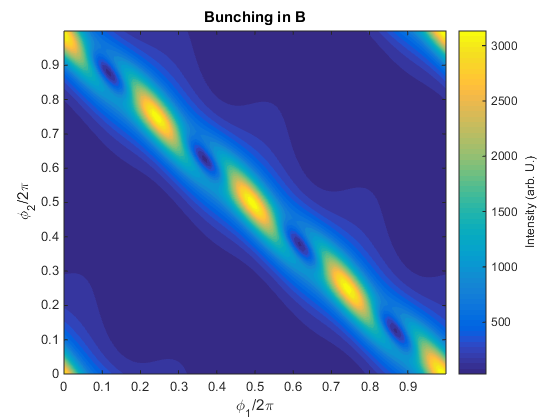
\includegraphics[width = \textwidth]{img/Bunching_B}
\caption{}
\end{subfigure}\,
\begin{subfigure}{0.49\textwidth}
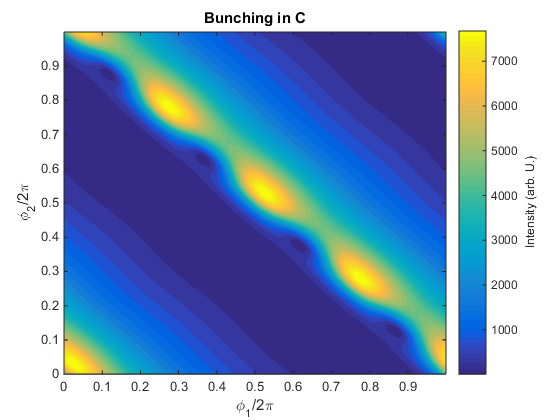
\includegraphics[width = \textwidth]{img/Bunching_C}
\caption{}
\end{subfigure}
\caption{Simulated probabilities (a) $|\beta_{bb}|^2$ and (b) $|\beta_{cc}|^2$ for the state $\ket{bb}$ and $\ket{cc}$ as a function of phases $\phi_1$ and $\phi_2$, not yet normalized. Credits to: Massimo Borghi}\label{bounchstates}
\end{figure}

\begin{figure}
\centering
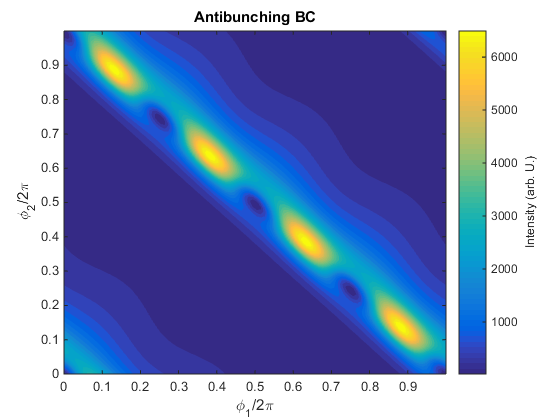
\includegraphics[width = .8\textwidth]{img/Antibunching_BC}
\caption{Simulated probability $|\beta_{bc}|^2$ for the state $\ket{bc}$ as a function of phases $\phi_1$ and $\phi_2$, not yet normalized. Credits to: Massimo Borghi}\label{antibounchstate}
\end{figure}

\section{Conclusion and further developments}
The calculation can go on, it is possibile to derive the power of the generated photons and also the rate. But the next important step is the experimental verification which is being performed by the nanoscience group of the University of Trento.\\
In this conclusion i want to dwell on the entanglement, which in this work is almost not present. The generated photon pairs are energy and time entangled, the fact that the energy is entangled can be seen from equation \eqref{conservationenergy} which express the conservation of energy of the generated photon. The sum of the frequencies of the generated photons is fixed, so if a photon have a determined frequency, the frequency of the other one is determined. The frequency is linked to energy by the Planck's constant $E = \hbar \omega$, so speaking about photons frequency is equal to speak about photon energy. The time entanglement is trickier to see, for this it is necessary to perform coincidence measurements. From the photodetection it can be seen that there is zero delay between the photons arrival, this means that the photons are emitted at the same time.\\
Lastly I want to thank Massimo Borghi for the great disponibility that he had for answering all my doubts and for all his help that I received for this thesis.

\bibliography{bibliography}
\bibliographystyle{plain}
\end{document} 
